\chapter{Appendix}
\label{apx:appendix}

\clearpage
\section{Structure of the Code Repository}
\dirtree{%
.1 code\DTcomment{Source code of our implementation}.
.2 00\_ARCHIVE\DTcomment{Archived resources from early experiments and analyses}.
.2 00\_CACHE\DTcomment{Cached resources like calculated event sync matrices}.
.2 00\_DATA.
.3 ERA\DTcomment{ERA-Interim dataset and download script}.
.3 TRMM\DTcomment{TRMM dataset and download script}.
.3 onset\_dates\_v2.csv\DTcomment{Onset dates as extracted from Singh}.
.2 00\_LOGS\DTcomment{Network training logs for analysis with tensorboard}.
.2 01\_ANALYSIS\DTcomment{Source for climate network analysis}.
.3 Dataset.py\DTcomment{Base class for both ERA and TRMM datasets}.
.3 ERA.py\DTcomment{Class for ERA-Interim processing}.
.3 TRMM.py\DTcomment{Class for TRMM processing}.
.3 Visualization.py\DTcomment{Class for creation of visualizations (cartopy)}.
.3 ERA \& TRMM.ipynb\DTcomment{Notebook with feature analysis}.
.3 Onset Dates.ipynb\DTcomment{Notebook with onset date analysis}.
.3 TRMM*.ipynb\DTcomment{Notebooks with TRMM climate network analysis}.
.2 02\_MODELLING\DTcomment{Source for onset prediction models}.
.3 LSTM\_E4.py\DTcomment{E4-Script with all configurations for the 45 basic experiments}.
.3 LSTM\_E4-final.py\DTcomment{E4-Script with the final repeated configurations}.
.3 models\DTcomment{Classes for the neural network models}.
.2 03\_EVALUATION\DTcomment{Evaluation results of neural network models}.
.3 histories\DTcomment{Training histories of experiments (csv files with loss/vloss)}.
.3 logs\DTcomment{Full training logs of experiments}.
.3 Accuracy Distributions.ipynb\DTcomment{Notebook with final model accuracy analysis}.
.2 *.sh\DTcomment{Shell scripts used for SLURM or PS experiments}.
.1 resources\DTcomment{Conda environment exports containing all important packages}.
.2 conda-*.env\DTcomment{Conda environments for windows pcs}.
.2 gru-*.env\DTcomment{Conda environments for linux machines}.
.1 thesis\DTcomment{Source code of the thesis and additional resources}.
.2 references.
.3 Experiments.xlsx\DTcomment{Results of all TRMM and ERA experiments}.
.3 TestAccuracy.csv\DTcomment{Predictions of all five final evaluations}.
.3 Visualizations.pptx\DTcomment{Visualizations as found in the thesis}.
}

\clearpage
\section{Monsoon Onset Dates}
\label{apx:onset_dates}

\begin{figure}[h]
  \centering
  \begin{tabular}{cc}
    \subfloat{
      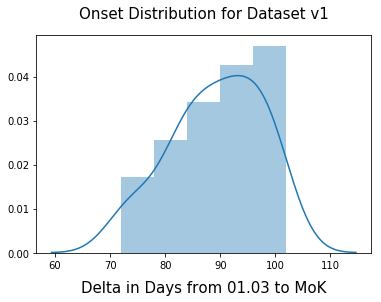
\includegraphics[width = 0.3\linewidth]{./99_appendix/img/onset_hist_v1}} &
    \subfloat{
      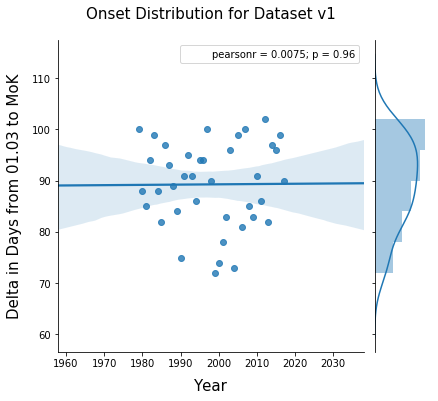
\includegraphics[width = 0.3\linewidth]{./99_appendix/img/onset_joint_v1}} \\
    \subfloat{
      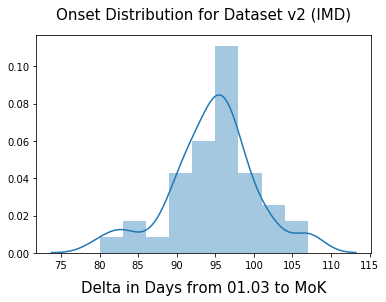
\includegraphics[width = 0.3\linewidth]{./99_appendix/img/onset_hist_v2_imd}} &
    \subfloat{
      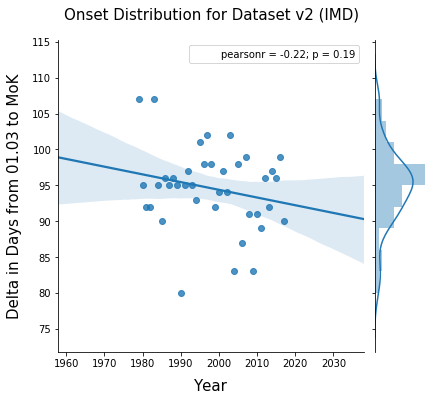
\includegraphics[width = 0.3\linewidth]{./99_appendix/img/onset_joint_v2_imd}} \\
    \subfloat{
      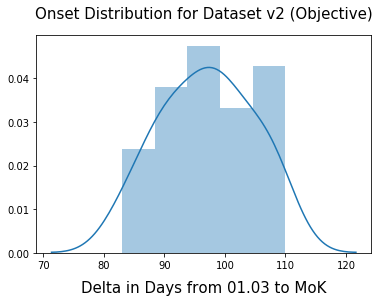
\includegraphics[width = 0.3\linewidth]{./99_appendix/img/onset_hist_v2_obj}} &
    \subfloat{
      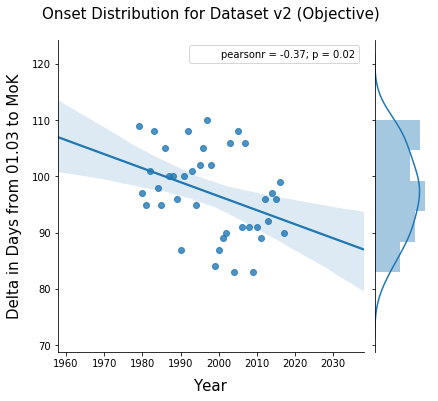
\includegraphics[width = 0.3\linewidth]{./99_appendix/img/onset_joint_v2_obj}} \\
  \end{tabular}
  \caption{Overview of Onset Distributions (1979-2017, v1: \citet{Ordonez.2016, IndiaMeteorologicalDepartment.2017b}, v2: \citet{Singh.2009, IndiaMeteorologicalDepartment.2017b}}
  \label{apx:onset_distributions}
\end{figure}

\begin{figure}[h]
  \centering
  \begin{tabular}{cc}
    \subfloat{
      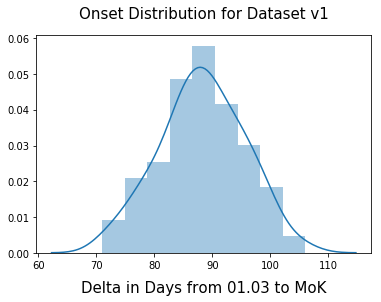
\includegraphics[width = 0.3\linewidth]{./99_appendix/img/onset_hist_v1_uncut}} &
    \subfloat{
      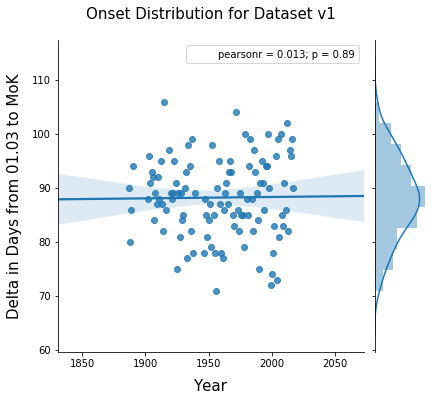
\includegraphics[width = 0.3\linewidth]{./99_appendix/img/onset_joint_v1_uncut}} \\
    \subfloat{
      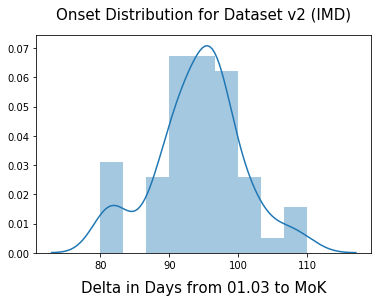
\includegraphics[width = 0.3\linewidth]{./99_appendix/img/onset_hist_v2_imd_uncut}} &
    \subfloat{
      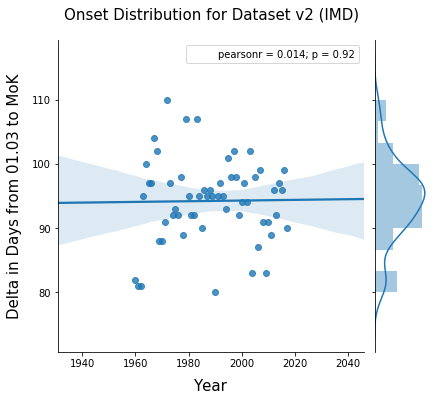
\includegraphics[width = 0.3\linewidth]{./99_appendix/img/onset_joint_v2_imd_uncut}} \\
    \subfloat{
      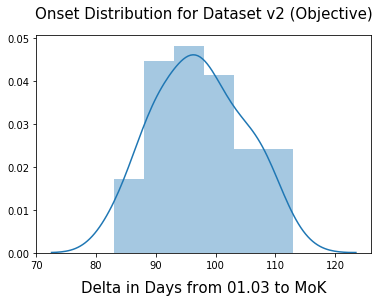
\includegraphics[width = 0.3\linewidth]{./99_appendix/img/onset_hist_v2_obj_uncut}} &
    \subfloat{
      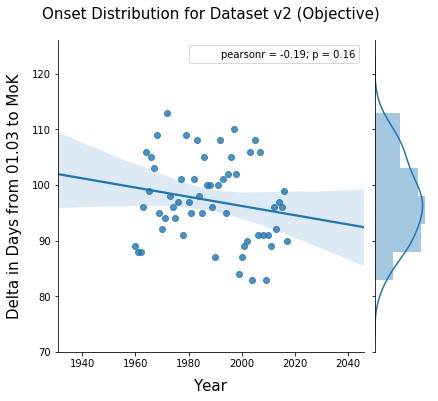
\includegraphics[width = 0.3\linewidth]{./99_appendix/img/onset_joint_v2_obj_uncut}} \\
  \end{tabular}
  \caption{Overview of Onset Distributions (v1: 1887-2017, \citet{Ordonez.2016, IndiaMeteorologicalDepartment.2017b}, v2: 1960-2017, \citet{Singh.2009, IndiaMeteorologicalDepartment.2017b})}
  \label{apx:onset_distributions_uncut}
\end{figure}

\clearpage
\section{TRMM \& ERA}
\label{apx:trmm_era}

\subsection{Getting the datasets}
\label{apx:download}
The process for downloading the TRMM dataset can be summarized as follows:
\begin{enumerate}
  \item Create an account for NASA Earthdata at \url{https://urs.earthdata.nasa.gov/home}
  \item Subset the TRMM dataset using \url{https://disc.gsfc.nasa.gov/SSW/#keywords=TRMM_3B42_Daily%207}
  \item Select the \textit{precipitation} variable (the aggregation of the other ones)
  \item Download the list of URLs in a file as offered in the subset results
  \item To download the dataset, follow the official instructions (especially setting the cookie) as offered in \url{https://disc.gsfc.nasa.gov/SSW/SSW_URL_List_Downloading_Instructions.html} (can be used in combination with our download script)
\end{enumerate}

The process for downloading of the ERA-Interim dataset is slightly more complex, as it requires the usage of an official library to download more than one month at a time. While the dataset could also be downloaded using \url{http://apps.ecmwf.int/datasets/data/interim-full-daily/levtype=sfc/}, this subset wizard only allows the download of one month at a time. The full process is structured as follows:
\begin{enumerate}
  \item Create an account for ECMWF data access at \url{https://apps.ecmwf.int/registration/}
  \item Follow the description as can be found on \url{https://software.ecmwf.int/wiki/display/WEBAPI/Access+ECMWF+Public+Datasets}
  \item Our download script is already setup to download all the ERA-Interim features used in this work. However, it assumes that dataset access has already been setup.
\end{enumerate}

\subsection{Usage with Python}
When it comes to handling meteorological datasets, there are two data formats one needs to know of. These formats, GRIB and NetCDF, store the datasets using optimized binary files and one needs a compatible library to read them. For NetCDF, such libraries are easy to find. The one we have found to work best is \textit{xarray}, which can be found at \url{http://xarray.pydata.org/en/stable/io.html}.

The xarray library would also allow reading in GRIB files when the additional \textit{PyNIO} library is installed. However, we have not been able to get PyNIO to work (or any other GRIB-related Python library, at that). TRMM and ERA-Interim both support the download of data using NetCDF and we would strongly suggest using this format whenever possible (at least when using Python).

\clearpage
\subsection{Feature analysis}
\label{apx:era_features}
The visualizations in this section show the development of different relevant ERA and TRMM features over the duration of an average monsoon. To calculate the visualizations, the data for each feature has been averaged over all years available (1998-2017 for TRMM, 1979-2017 for ERA).

\textbf{Example:} The temperature grids 10 days previous to the objective onset dates (MoK; \ref{apx:era_t}) for all available years are extracted and then averaged to yield an averaged grid representation. The visualization is then simply calculated based on the averaged grid.

\begin{figure}[h]
  \centering
  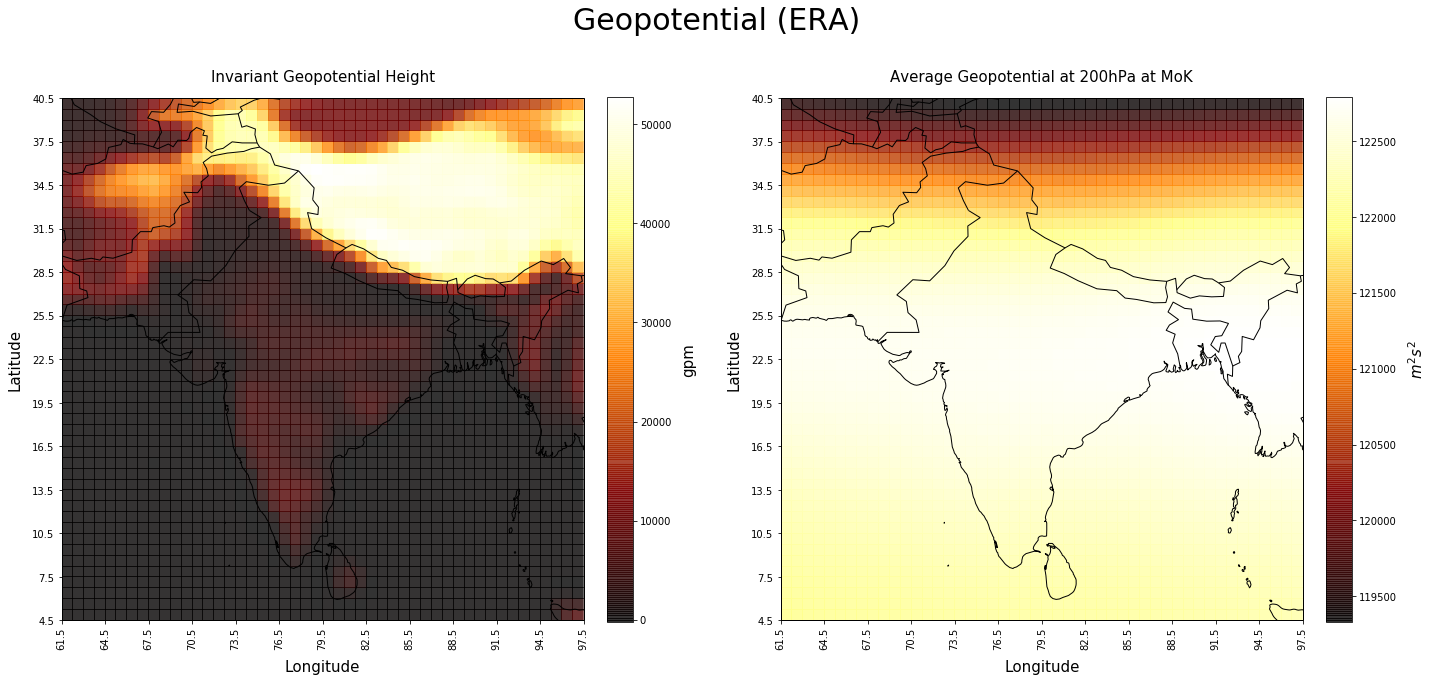
\includegraphics[width=\linewidth]{./99_appendix/img/geopotential}
  \caption{Geopotential Height and Geopotential at 200hPa (ERA-Interim, 1979-2017)}
  \label{apx:era_geopotential}
\end{figure}

\begin{figure}[h]
  \centering
  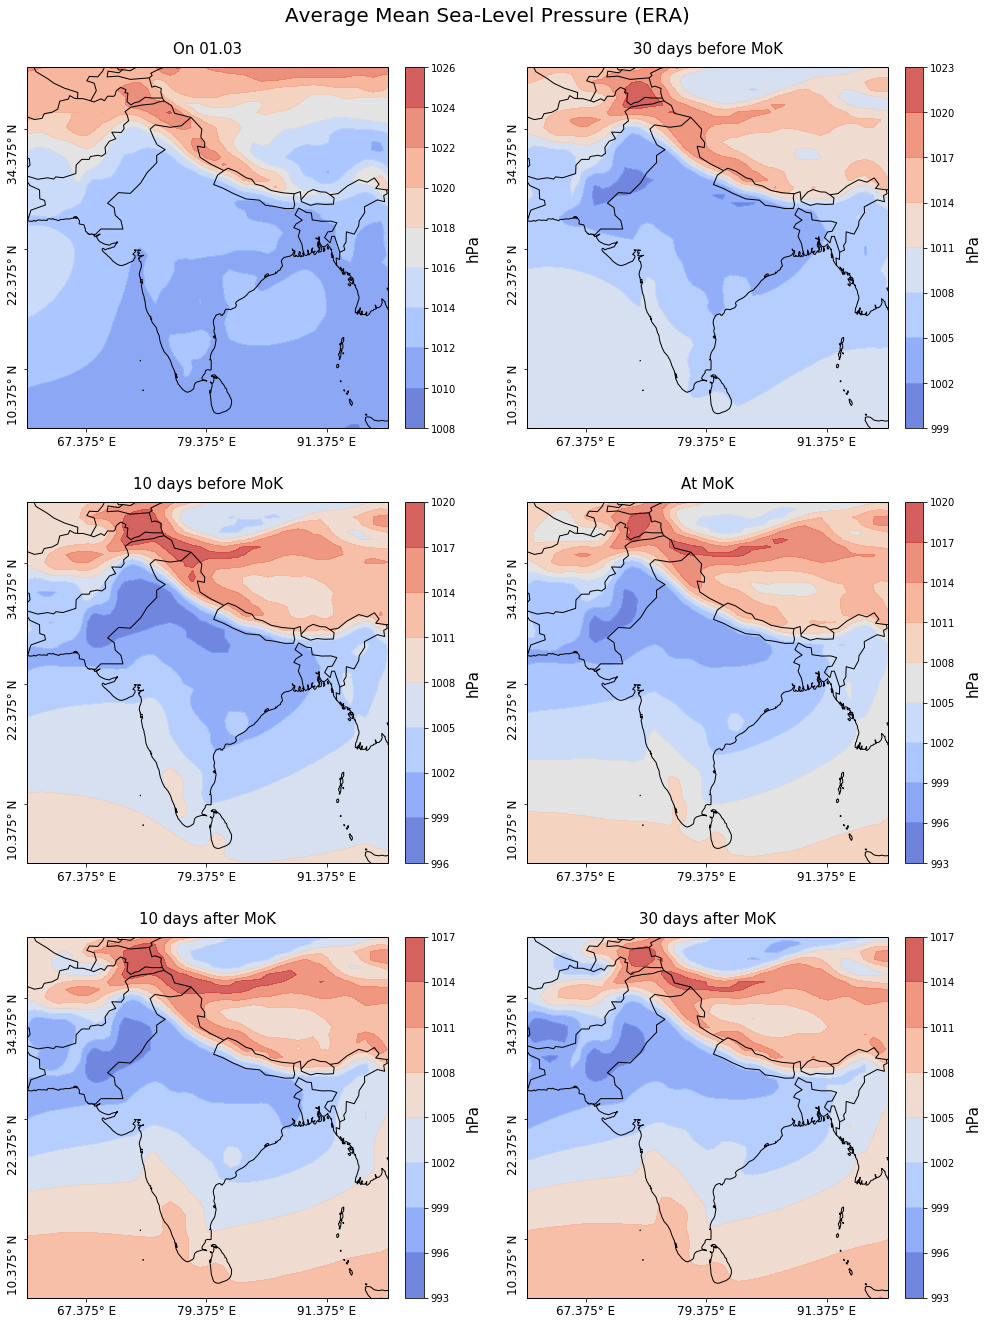
\includegraphics[width=\linewidth]{./99_appendix/img/msl_avg}
  \caption{Average Mean Sea-Level Pressure (ERA-Interim, 1979-2017)}
  \label{apx:era_msl}
\end{figure}

\begin{figure}[h]
  \centering
  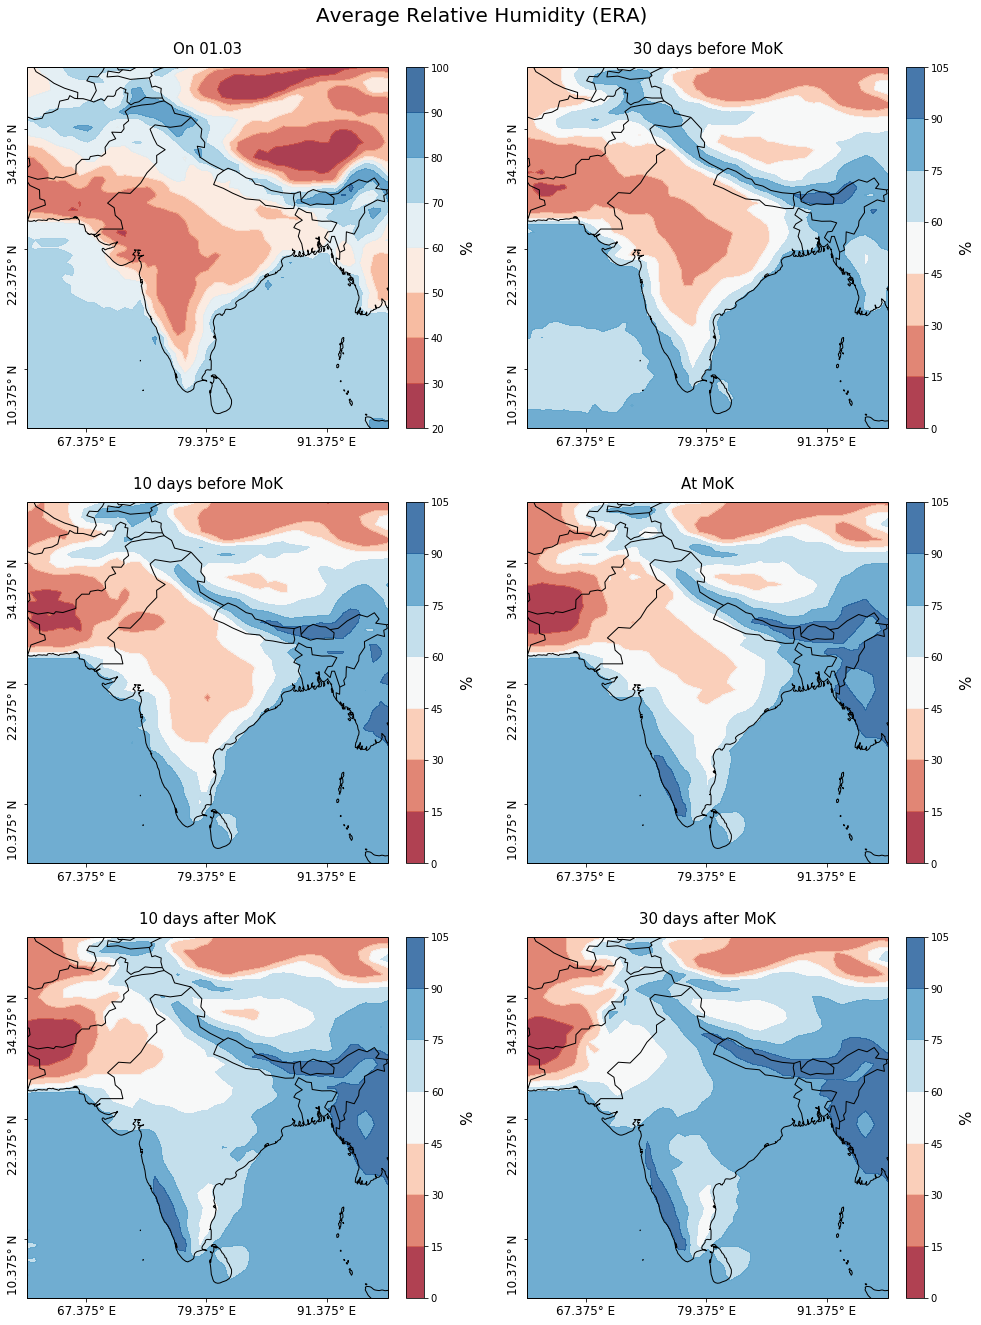
\includegraphics[width=\linewidth]{./99_appendix/img/r_avg}
  \caption{Average Relative Humidity at 1000hPa (ERA-Interim, 1979-2017)}
  \label{apx:era_r}
\end{figure}

\begin{figure}[h]
  \centering
  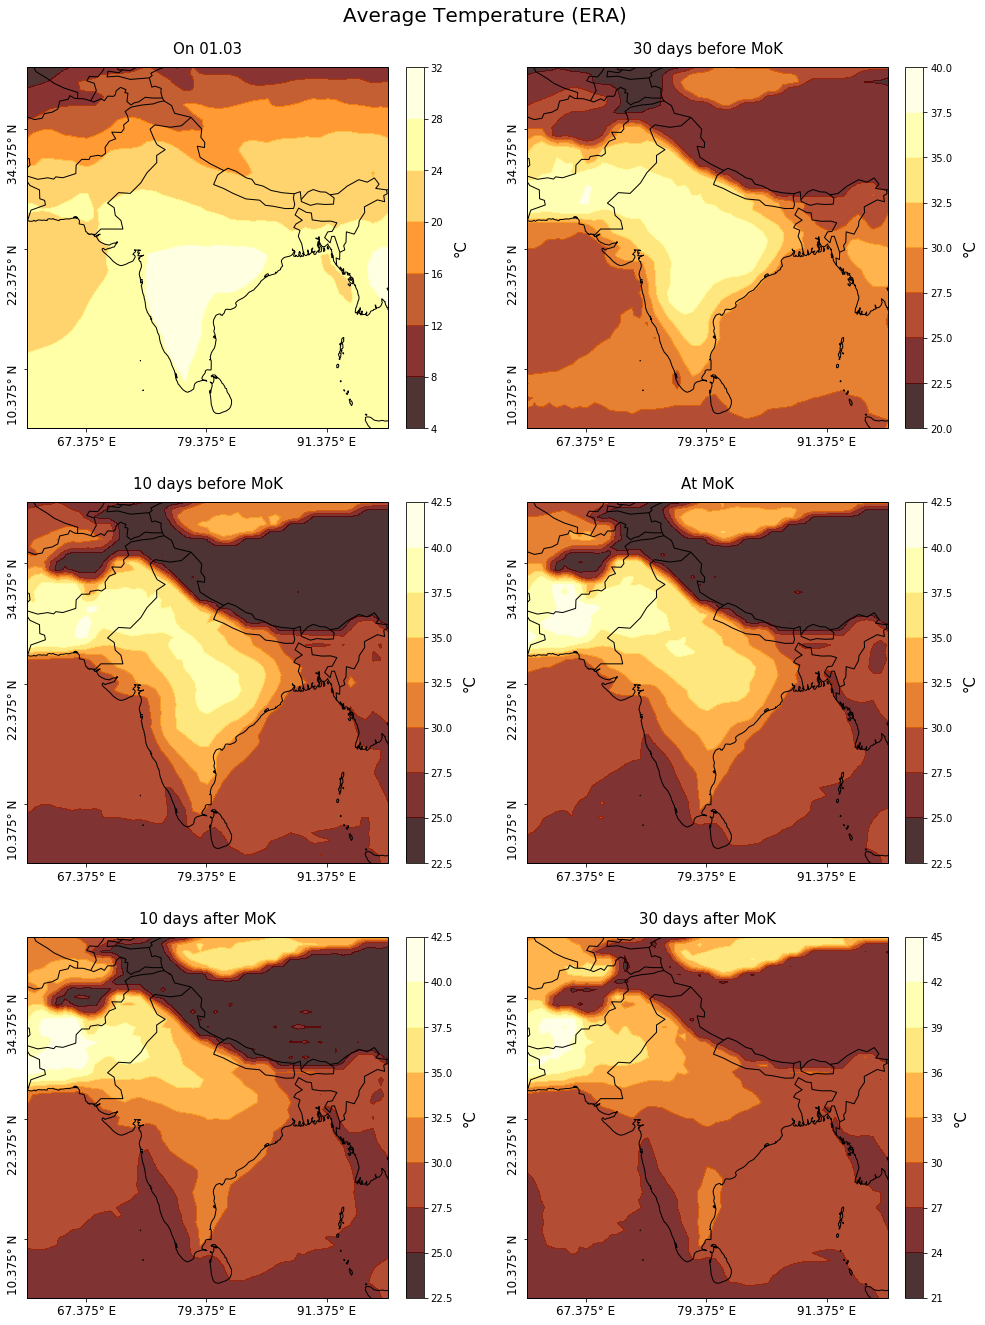
\includegraphics[width=\linewidth]{./99_appendix/img/t_avg}
  \caption{Average Temperature at 1000hPa (ERA-Interim, 1979-2017)}
  \label{apx:era_t}
\end{figure}

\begin{figure}[h]
  \centering
  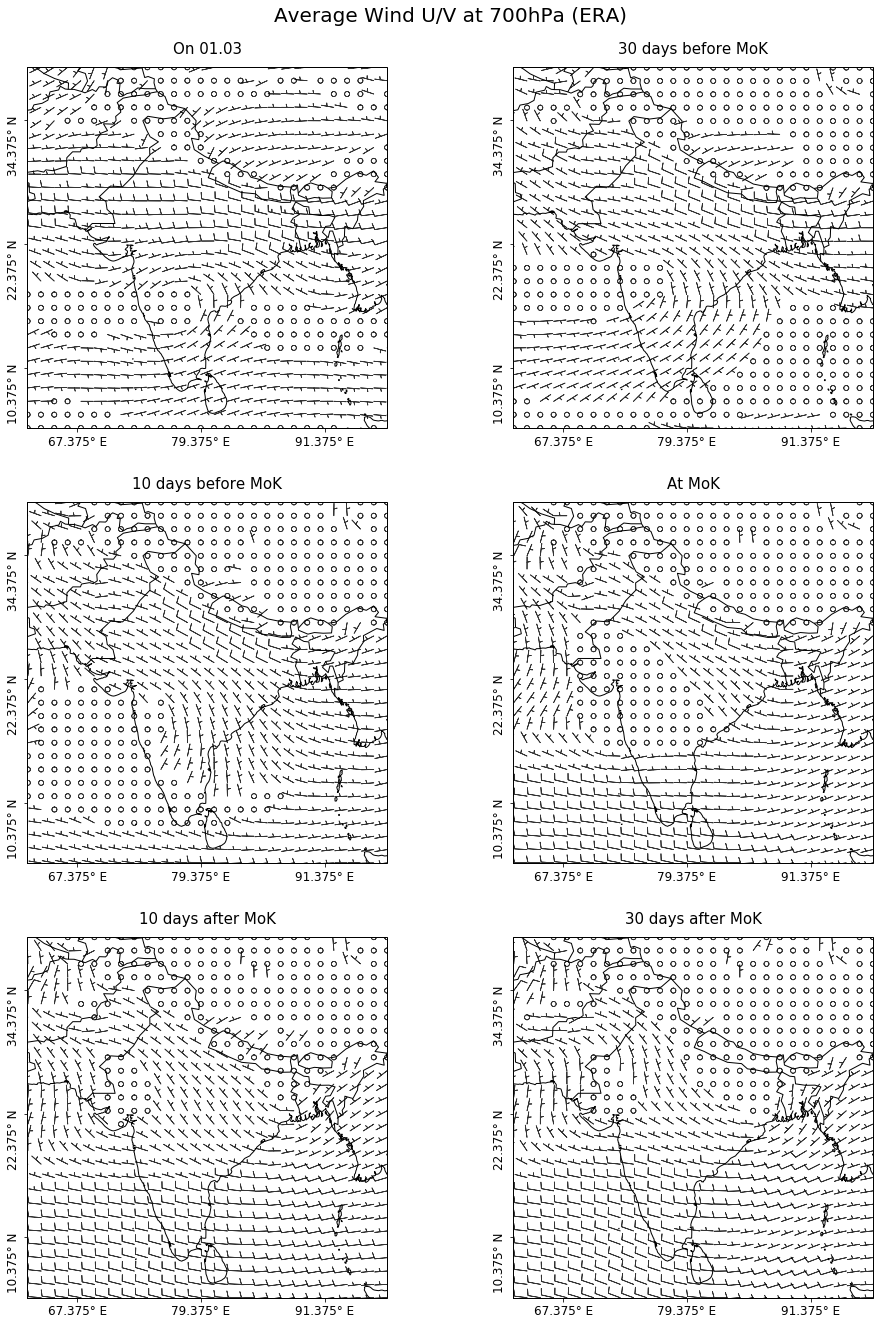
\includegraphics[width=\linewidth]{./99_appendix/img/wind_avg}
  \caption{Average Wind (U/V) at 700hPa (ERA-Interim, 1979-2017)}
  \label{apx:era_wind}
\end{figure}

\begin{figure}[h]
  \centering
  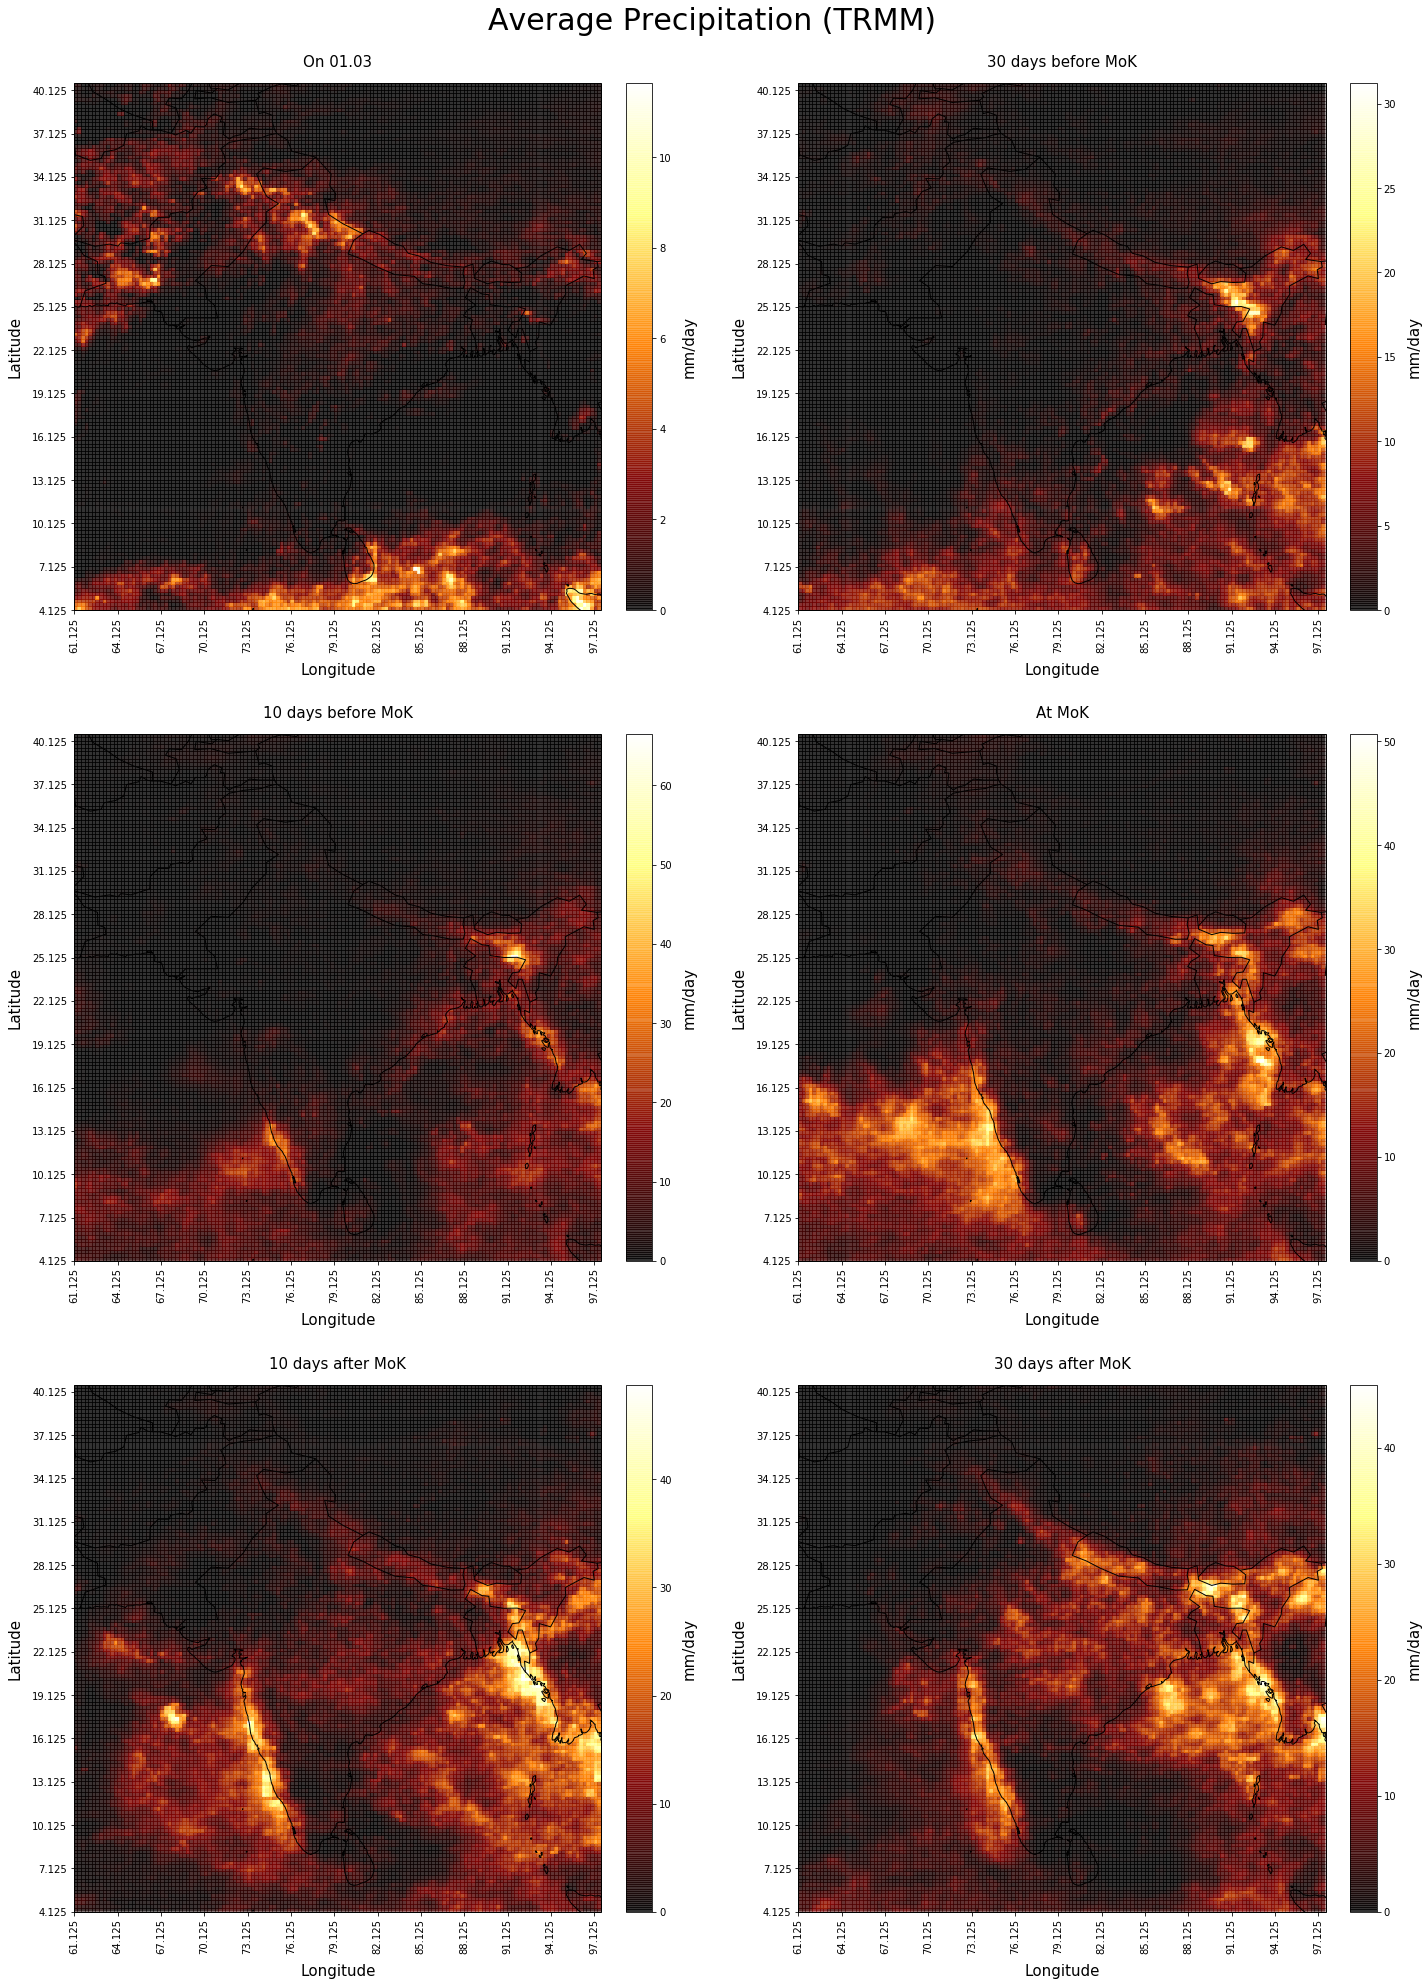
\includegraphics[width=\linewidth]{./99_appendix/img/prec_avg}
  \caption{Average Precipitation (TRMM, 1998-2017)}
  \label{apx:trmm_prec}
\end{figure}

\clearpage
\section{Event Synchronization}
\label{apx:event_sync}

\begin{figure}[h]
  \centering
  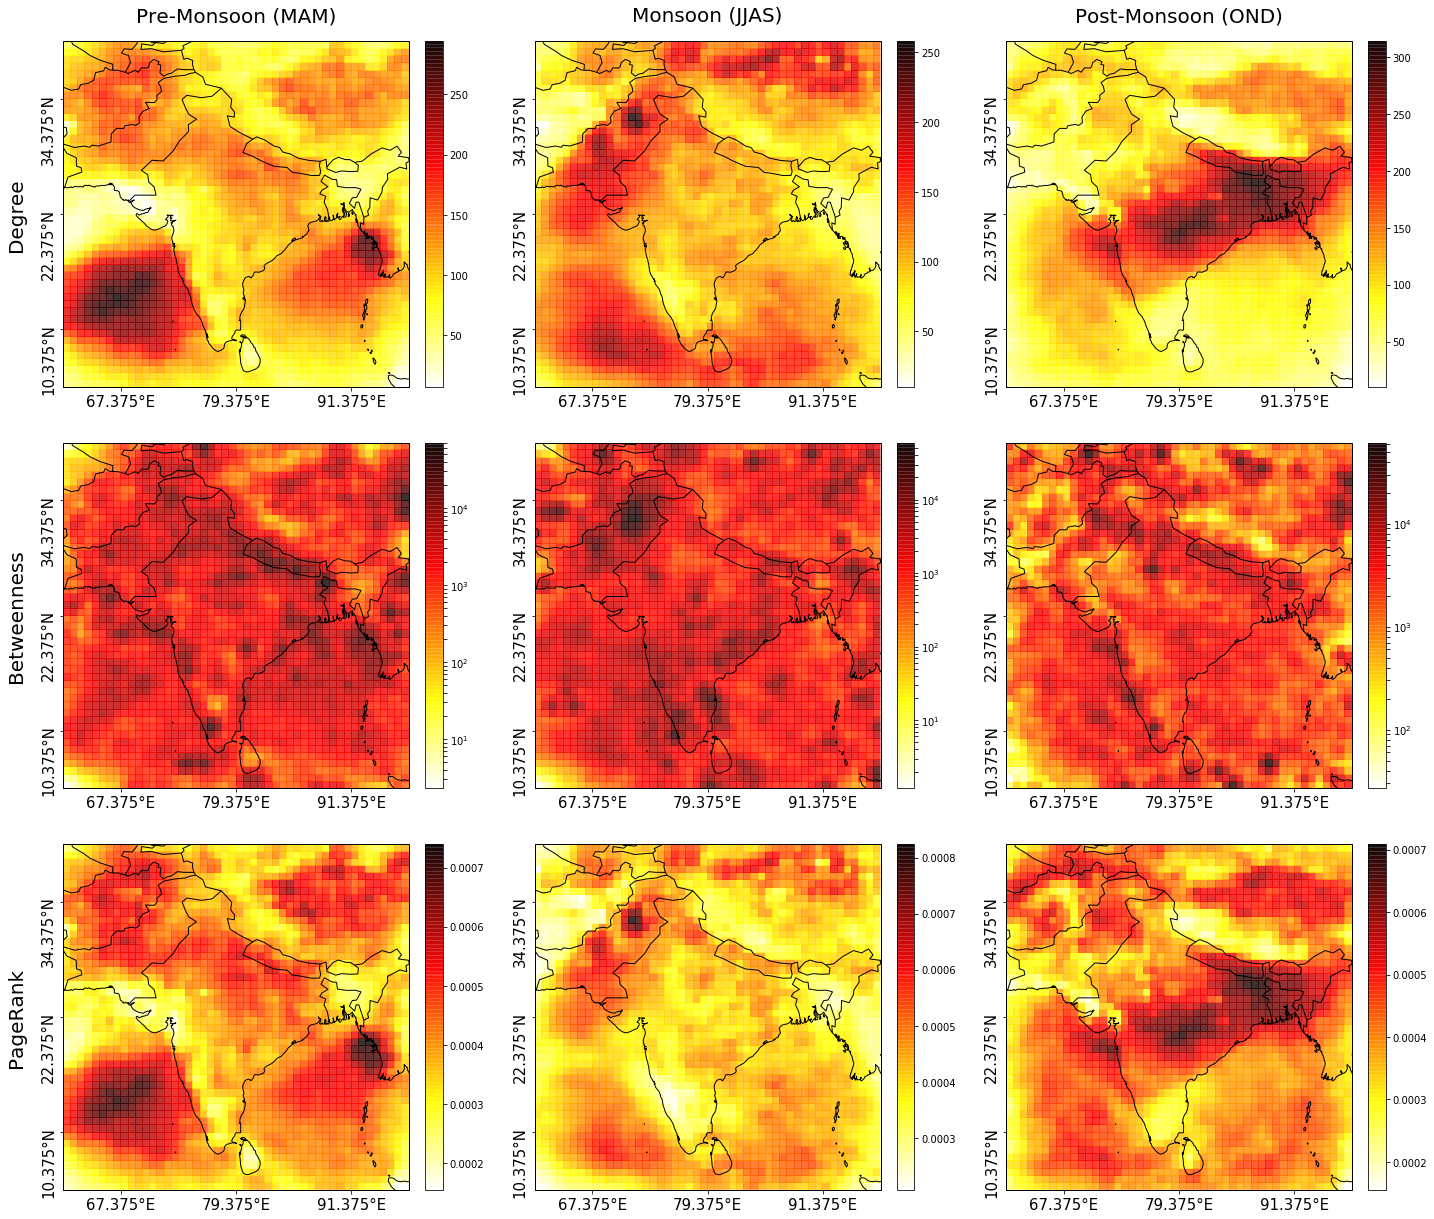
\includegraphics[width=\linewidth]{{./99_appendix/img/event_sync_0.75-0.9}.png}
  \caption{Climate network analysis for unweighted, undirected climate networks (based on TRMM at {0.75\degree} resolution and a threshold set at the 95th percentile).}
  \label{apx:climate_network_basic}
\end{figure}

\begin{figure}[h]
  \centering
  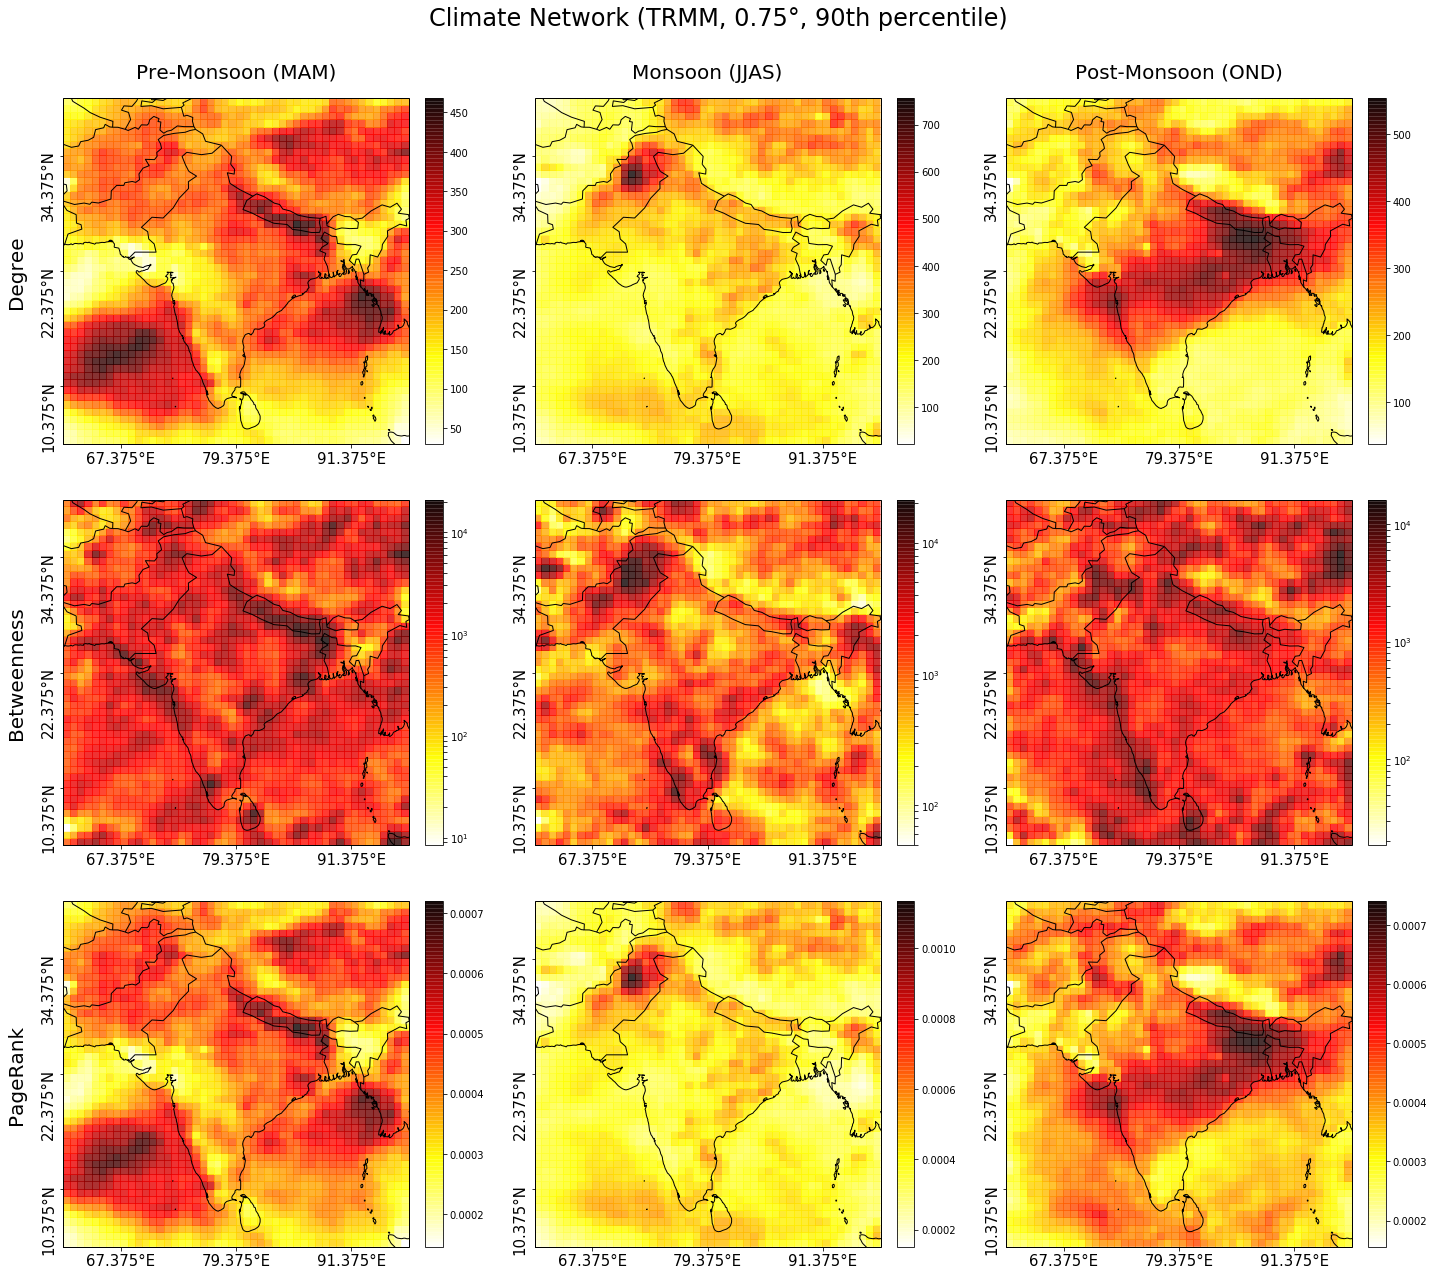
\includegraphics[width=\linewidth]{{./99_appendix/img/event_sync_0.75-0.9_90}.png}
  \caption{Climate network analysis for unweighted, undirected climate networks (based on TRMM at {0.75\degree} resolution and a threshold set at the 90th percentile).}
  \label{apx:climate_network_basic_90}
\end{figure}

\begin{figure}[h]
  \centering
  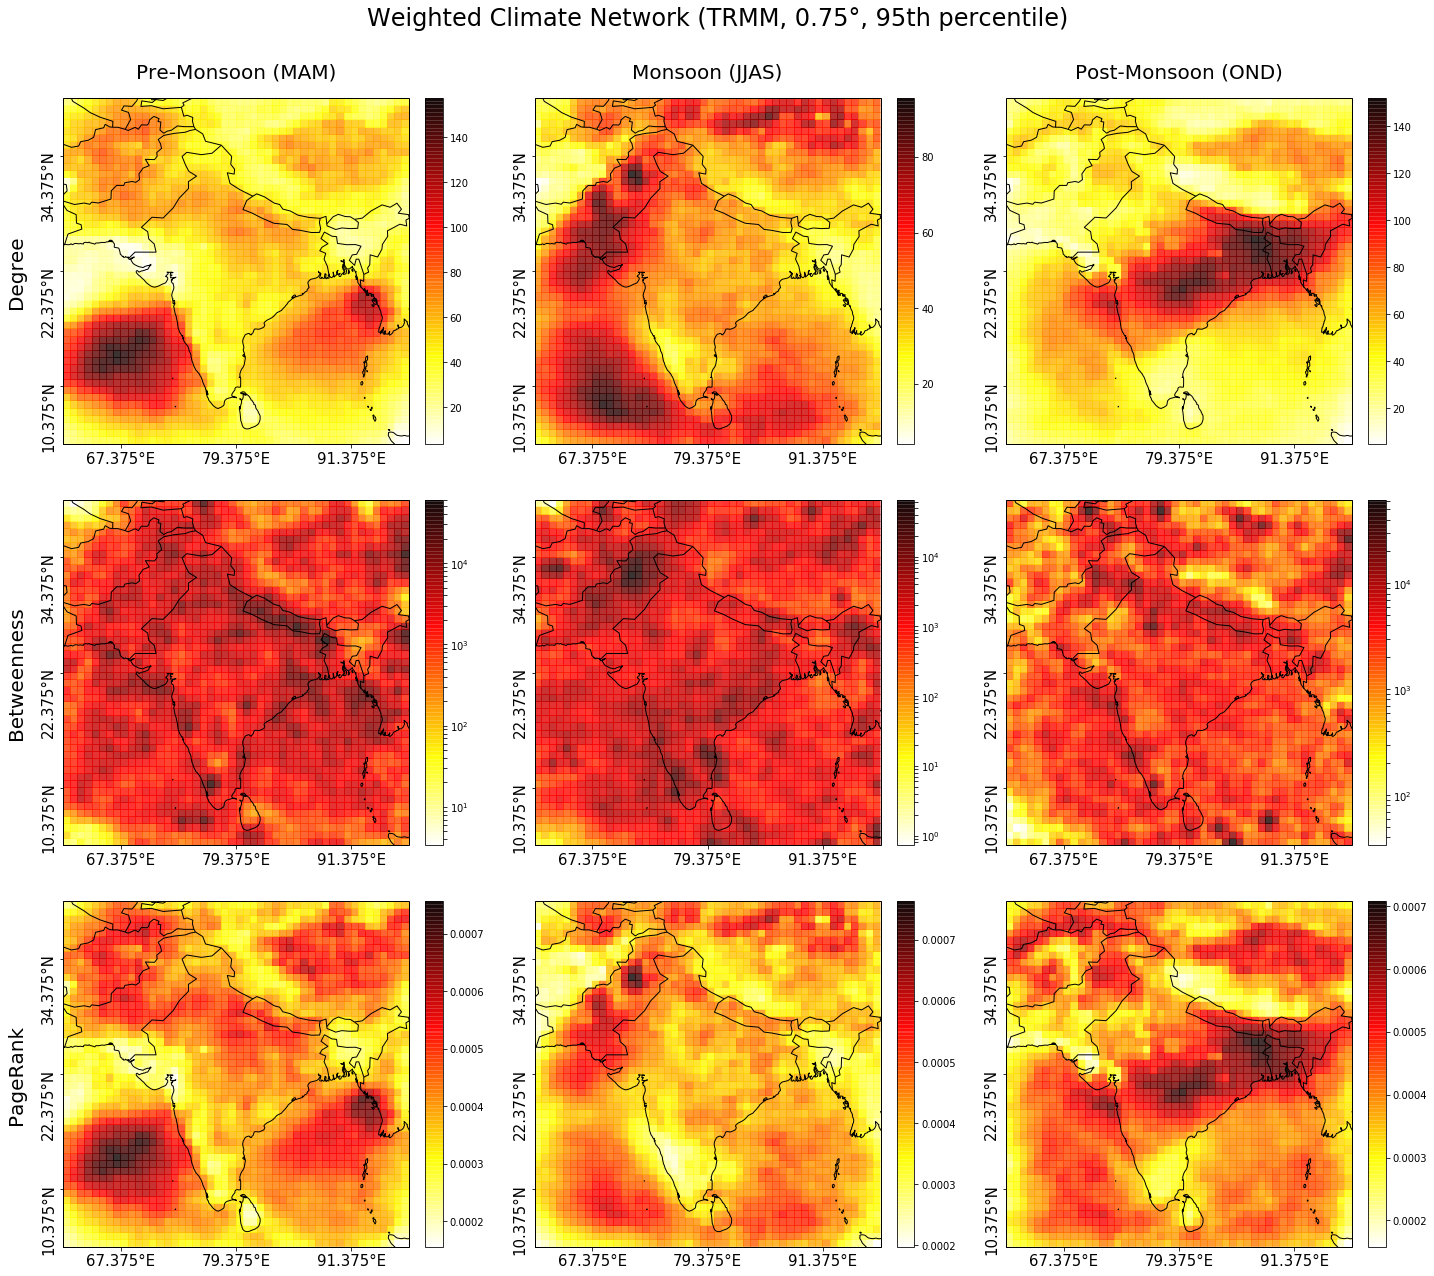
\includegraphics[width=\linewidth]{{./99_appendix/img/event_sync_0.75-0.9_weighted}.png}
  \caption{Climate network analysis for weighted, undirected climate networks (based on TRMM at {0.75\degree} resolution and a threshold set at the 95th percentile).}
  \label{apx:climate_network_weighted}
\end{figure}

\begin{figure}[h]
  \centering
  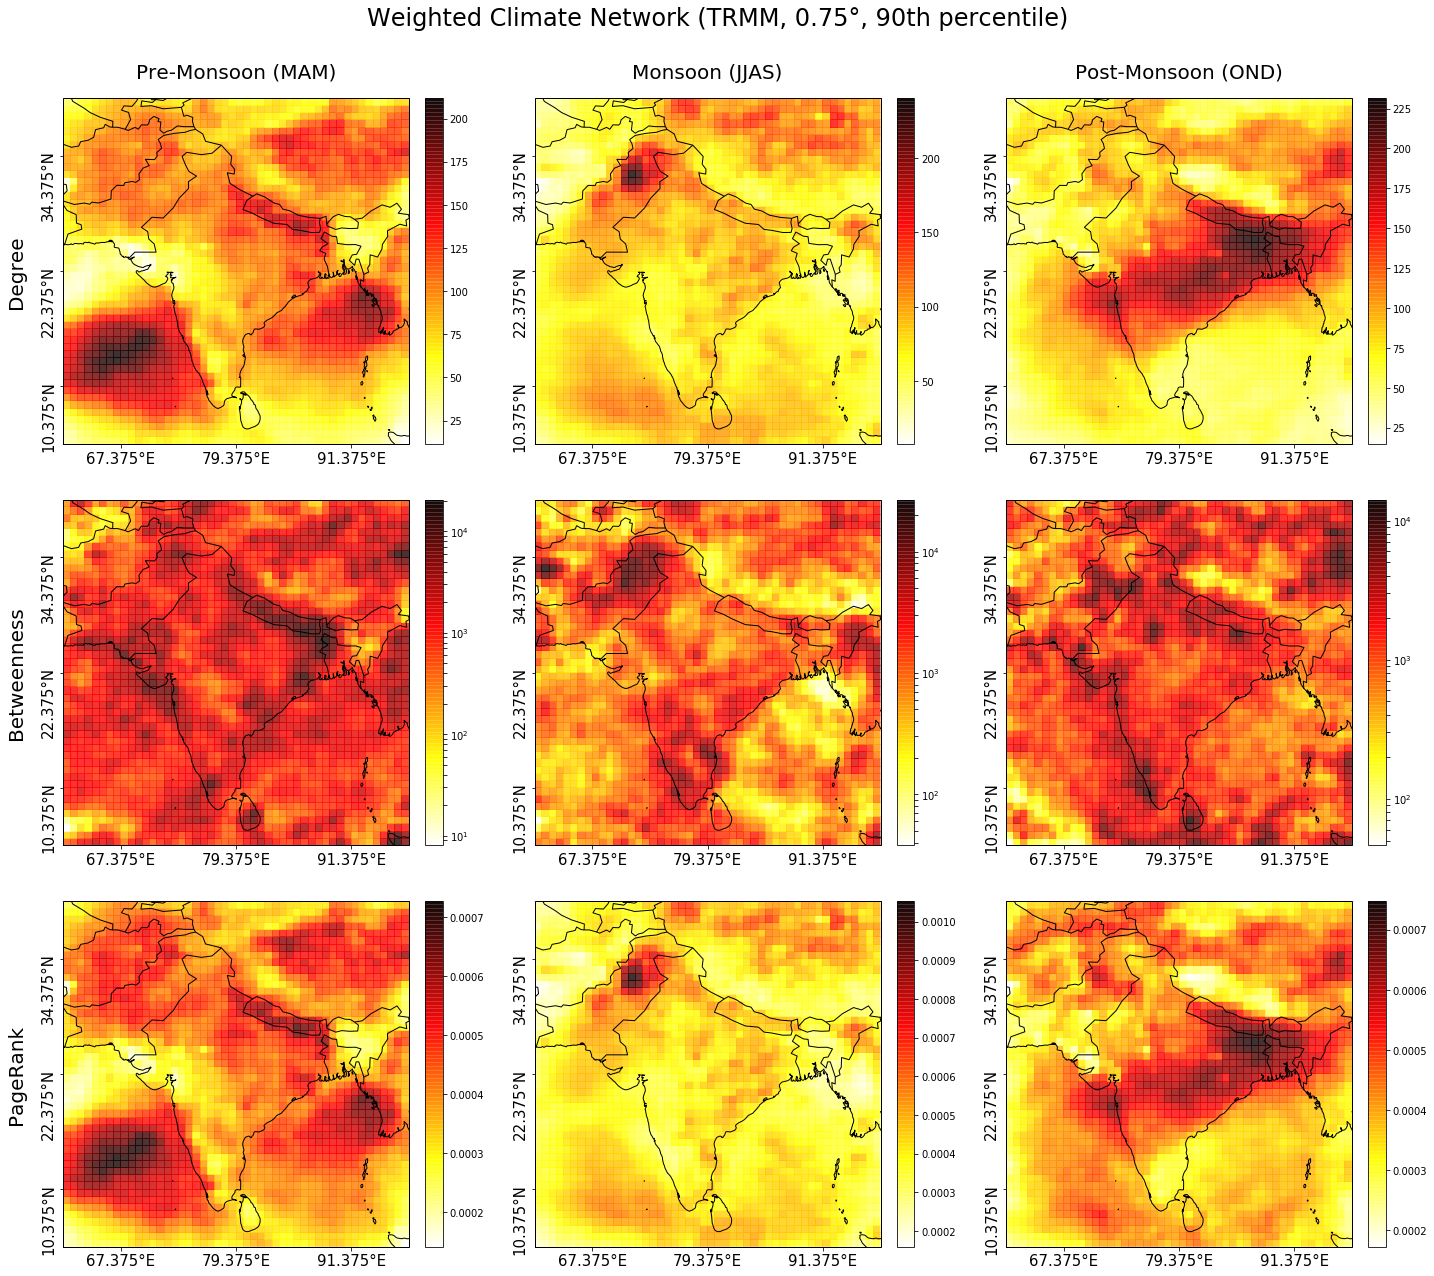
\includegraphics[width=\linewidth]{{./99_appendix/img/event_sync_0.75-0.9_weighted_90}.png}
  \caption{Climate network analysis for weighted, undirected climate networks (based on TRMM at {0.75\degree} resolution and a threshold set at the 90th percentile).}
  \label{apx:climate_network_weighted_90}
\end{figure}

\begin{figure}[h]
  \centering
  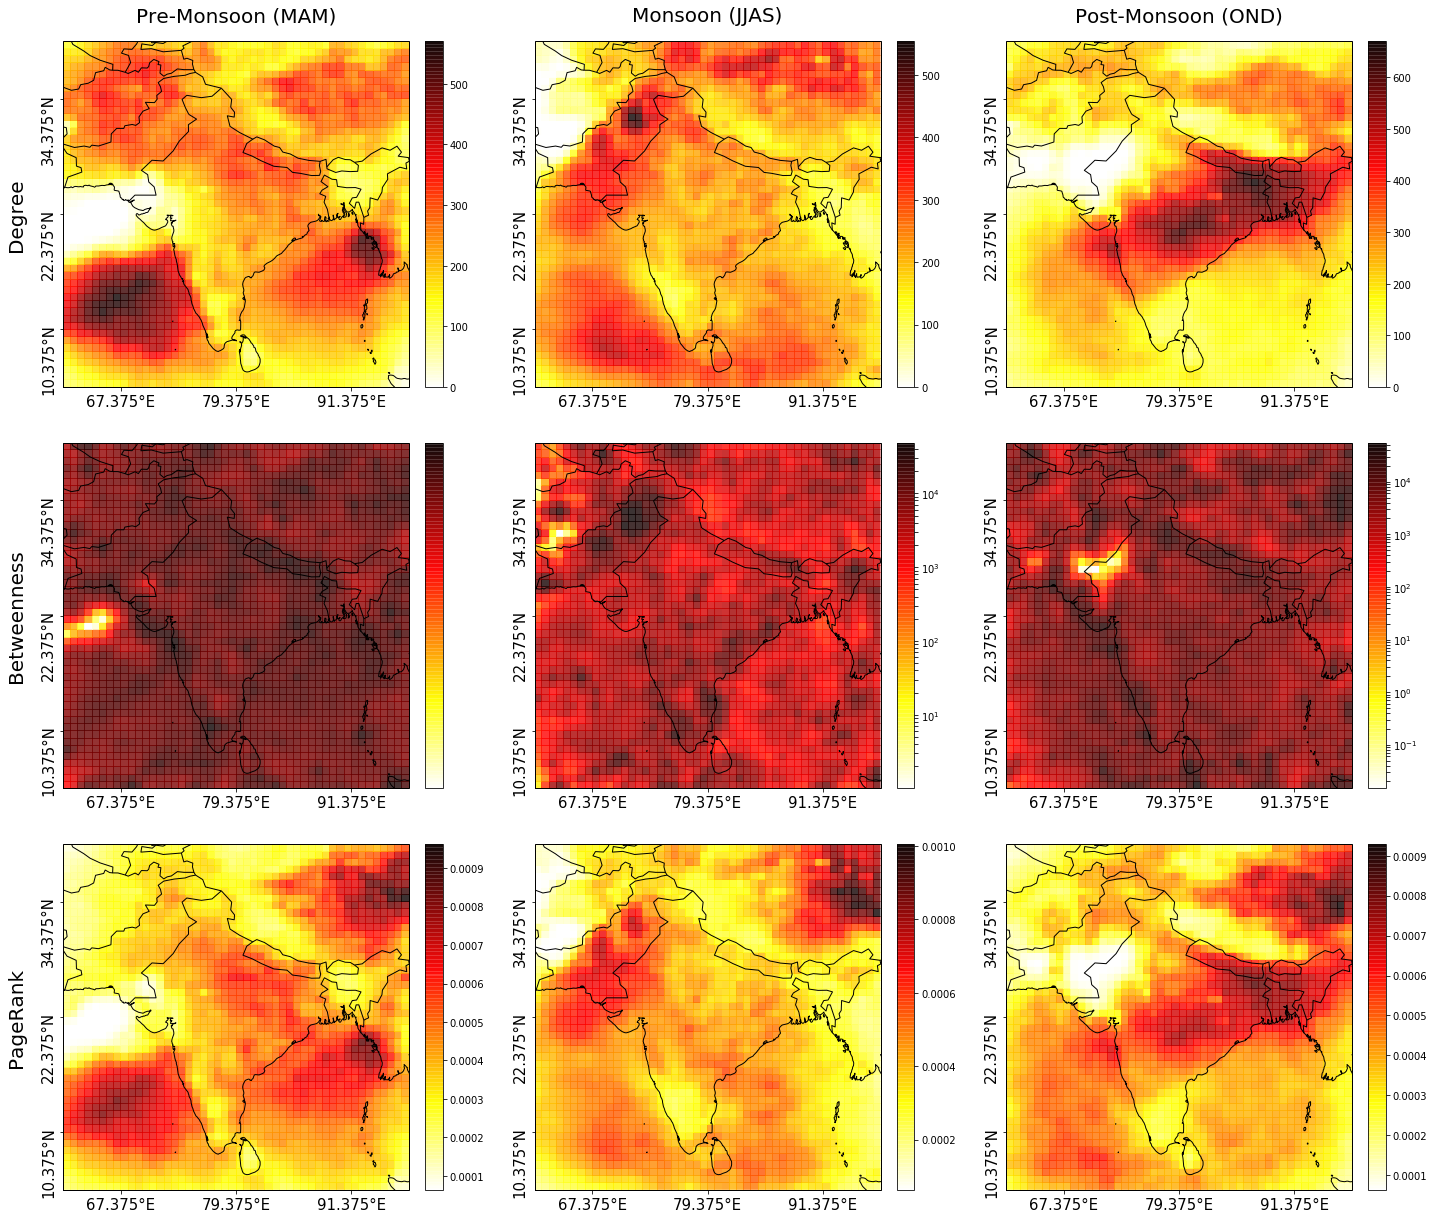
\includegraphics[width=\linewidth]{{./99_appendix/img/event_sync_0.75-0.9_directed}.png}
  \caption{Climate network analysis for unweighted, directed climate networks (based on TRMM at {0.75\degree} resolution and a threshold set at the 95th percentile).}
  \label{apx:climate_network_directed}
\end{figure}

\begin{figure}[h]
  \centering
  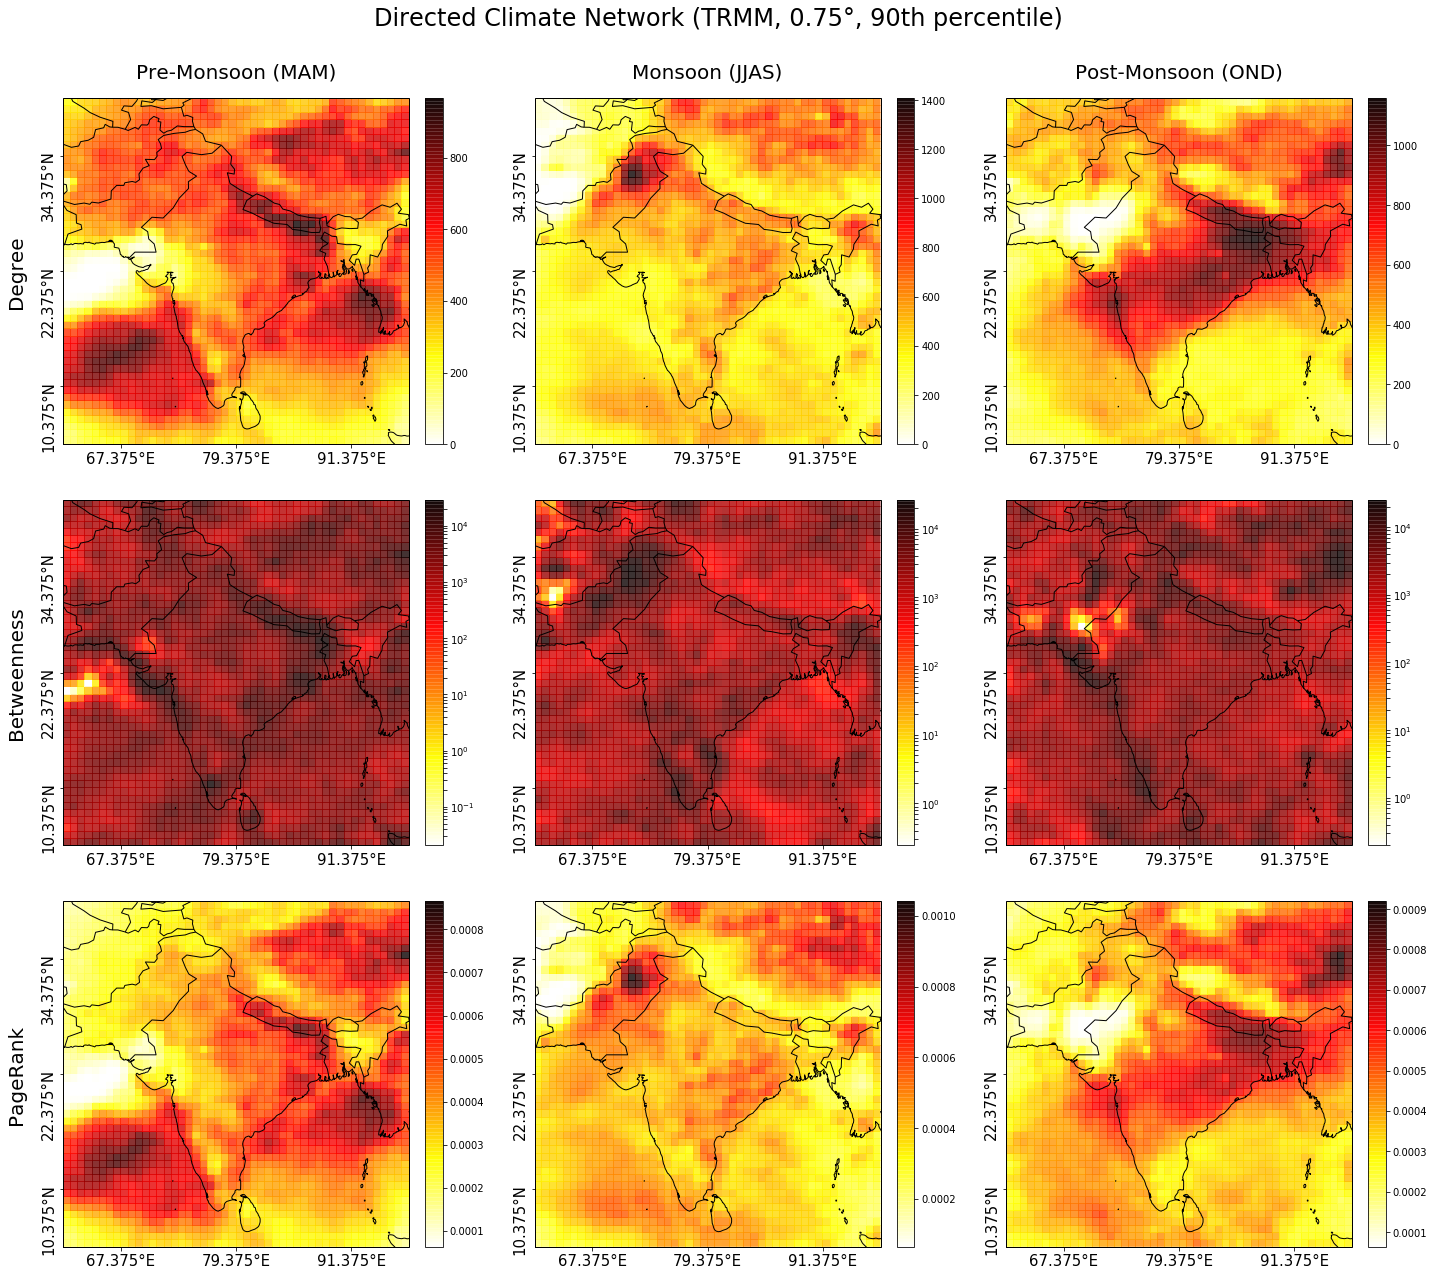
\includegraphics[width=\linewidth]{{./99_appendix/img/event_sync_0.75-0.9_directed_90}.png}
  \caption{Climate network analysis for unweighted, directed climate networks (based on TRMM at {0.75\degree} resolution and a threshold set at the 90th percentile).}
  \label{apx:climate_network_directed}
\end{figure}

\begin{figure}[h]
  \centering
  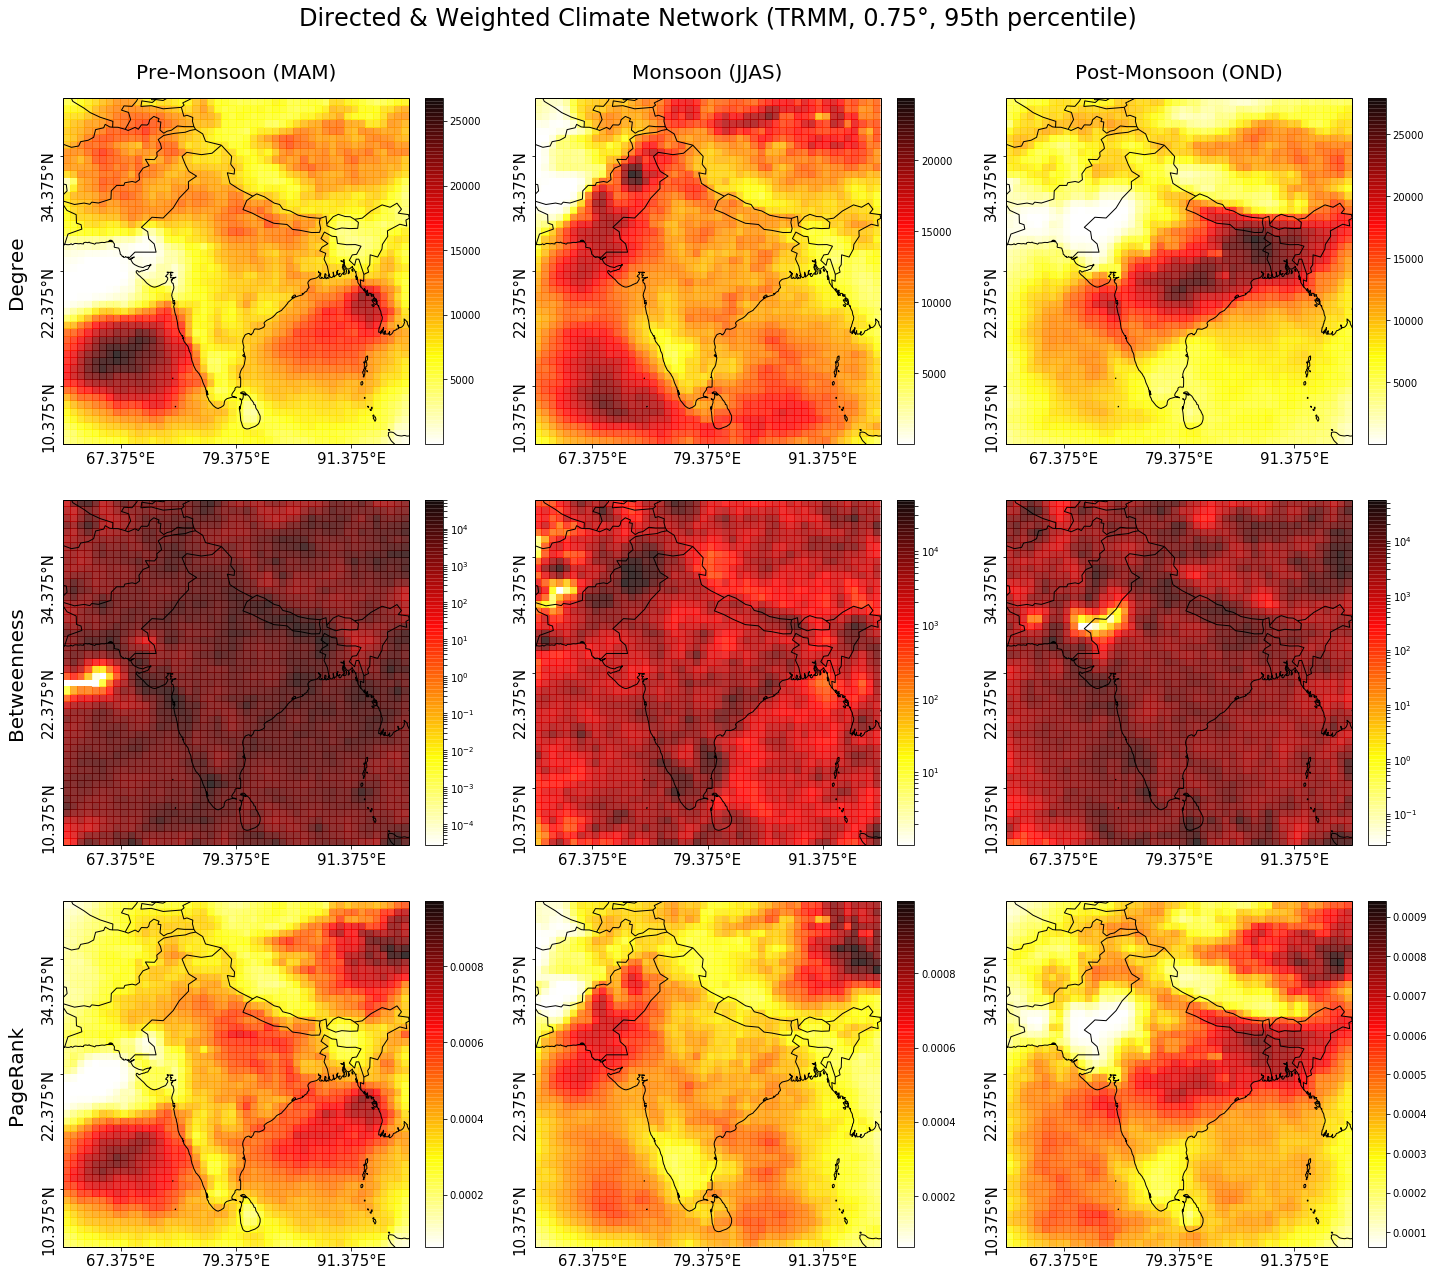
\includegraphics[width=\linewidth]{{./99_appendix/img/event_sync_0.75-0.9_directed_weighted}.png}
  \caption{Climate network analysis for weighted, directed climate networks (based on TRMM at {0.75\degree} resolution and a threshold set at the 95th percentile).}
  \label{apx:climate_network_both}
\end{figure}

\begin{figure}[h]
  \centering
  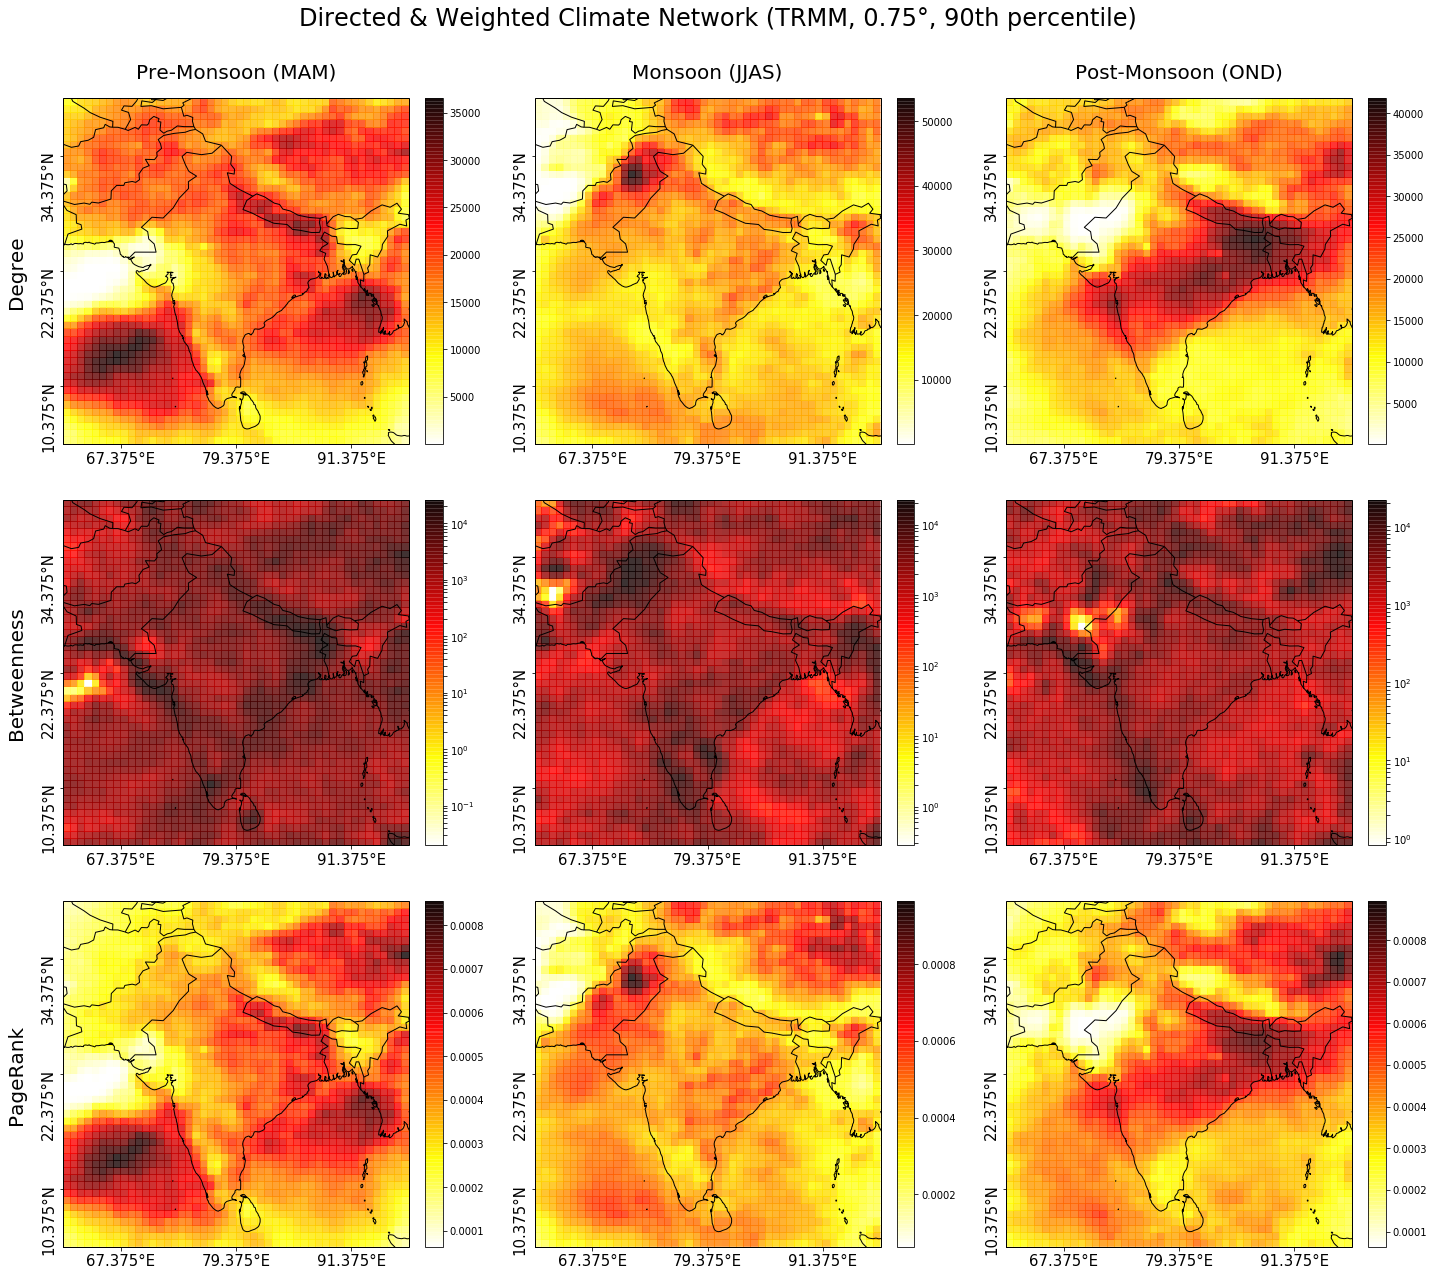
\includegraphics[width=\linewidth]{{./99_appendix/img/event_sync_0.75-0.9_directed_weighted_90}.png}
  \caption{Climate network analysis for weighted, directed climate networks (based on TRMM at {0.75\degree} resolution and a threshold set at the 90th percentile).}
  \label{apx:climate_network_both}
\end{figure}

\clearpage
\section{Neural Network Results}
\label{apx:nn_evaluation}

\begin{figure}[h]
  \centering
  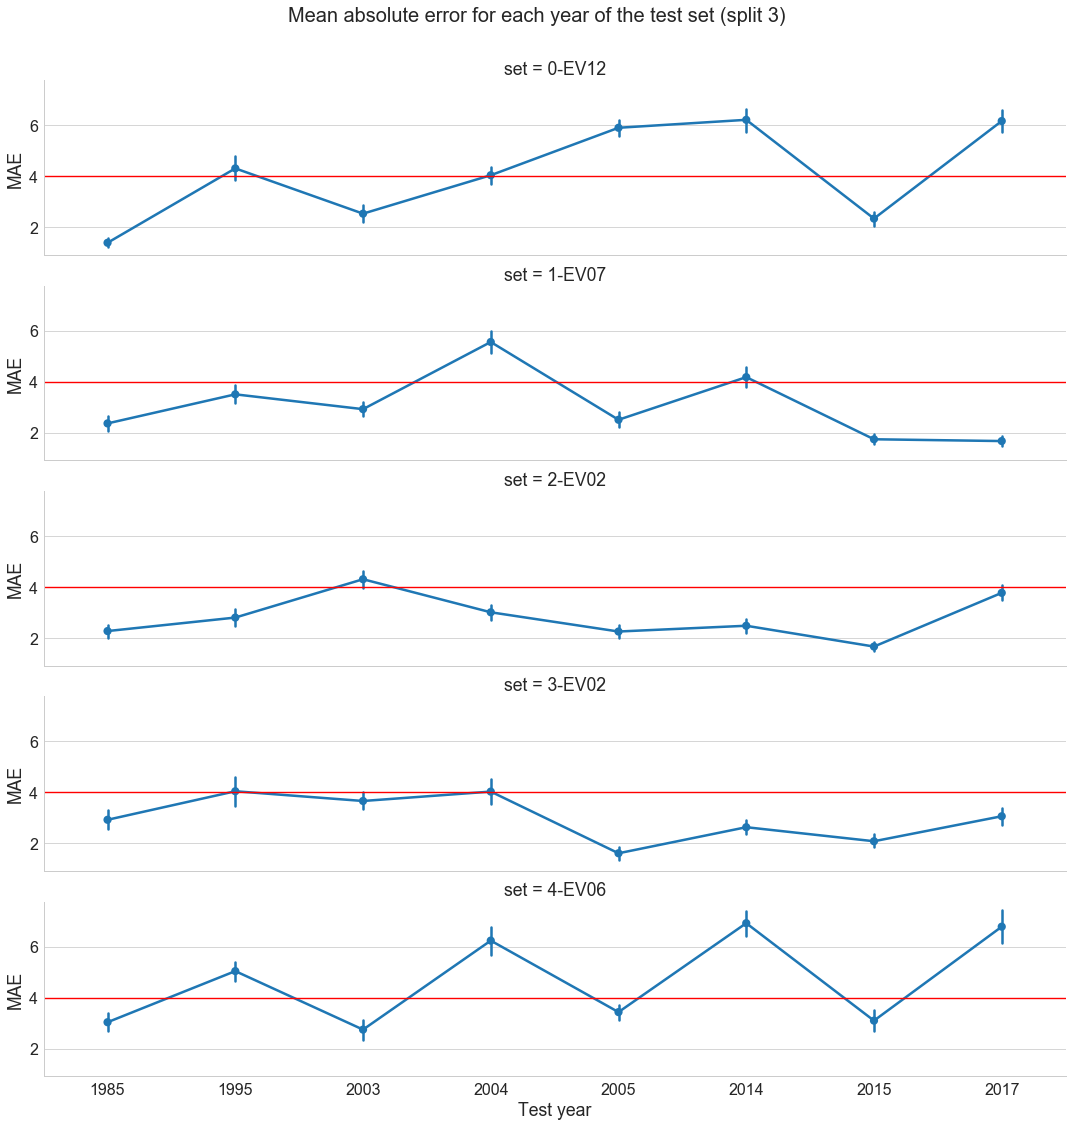
\includegraphics[width=0.9\linewidth]{./99_appendix/img/prediction_years_ci.png}
  \caption{Yearly mean-absolute error (with 0.95 CI) averaged over the predictions of the final experiments on the test set (1985, 1995, 2003, 2004, 2005, 2014, 2015, 2017).}
  \label{apx:prediction_years_ci}
\end{figure}

\begin{figure}[h]
  \centering
  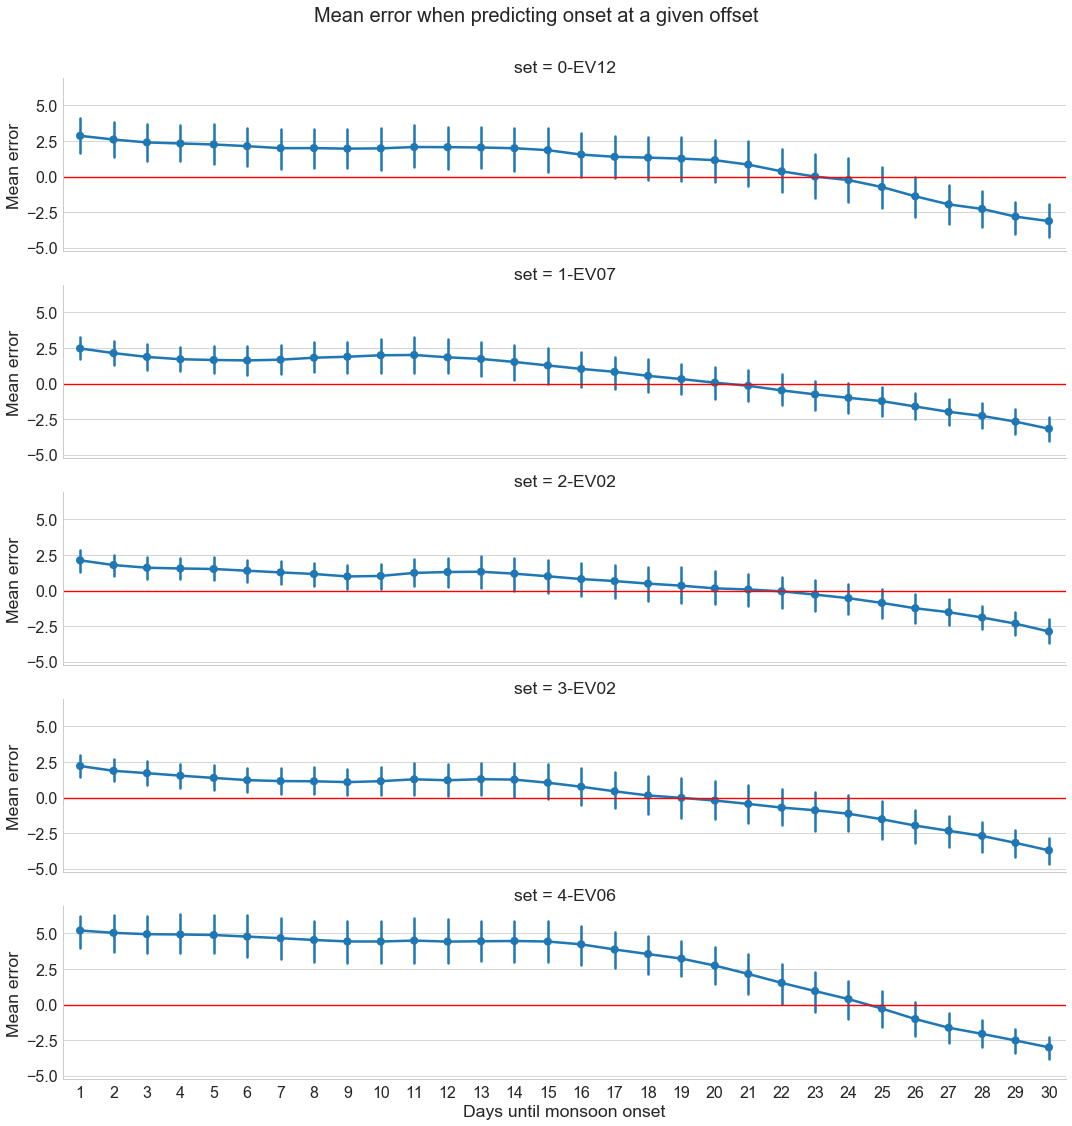
\includegraphics[width=0.9\linewidth]{./99_appendix/img/prediction_error_offset_split.png}
  \caption{Mean error (with 0.95 CI) of each offset from MoK, averaged over the predictions of the final experiments on the test set (1985, 1995, 2003, 2004, 2005, 2014, 2015, 2017).}
  \label{apx:prediction_error_offset_ci}
\end{figure}

\begin{figure}[h]
  \centering
  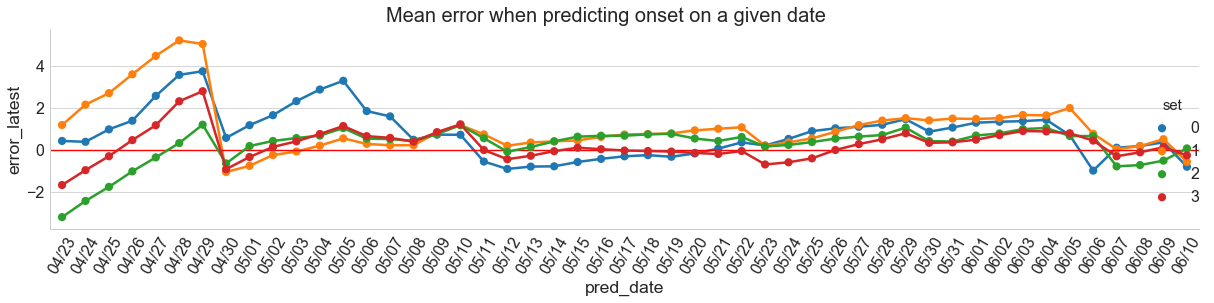
\includegraphics[width=\linewidth]{./99_appendix/img/prediction_error_dates.png}
  \caption{Mean error (with 0.95 CI) of each prediction date previous to MoK, averaged over the predictions of the final experiments on the test set (1985, 1995, 2003, 2004, 2005, 2014, 2015, 2017).}
  \label{apx:prediction_error_dates_ci}
\end{figure}

\begin{figure}[h]
  \centering
  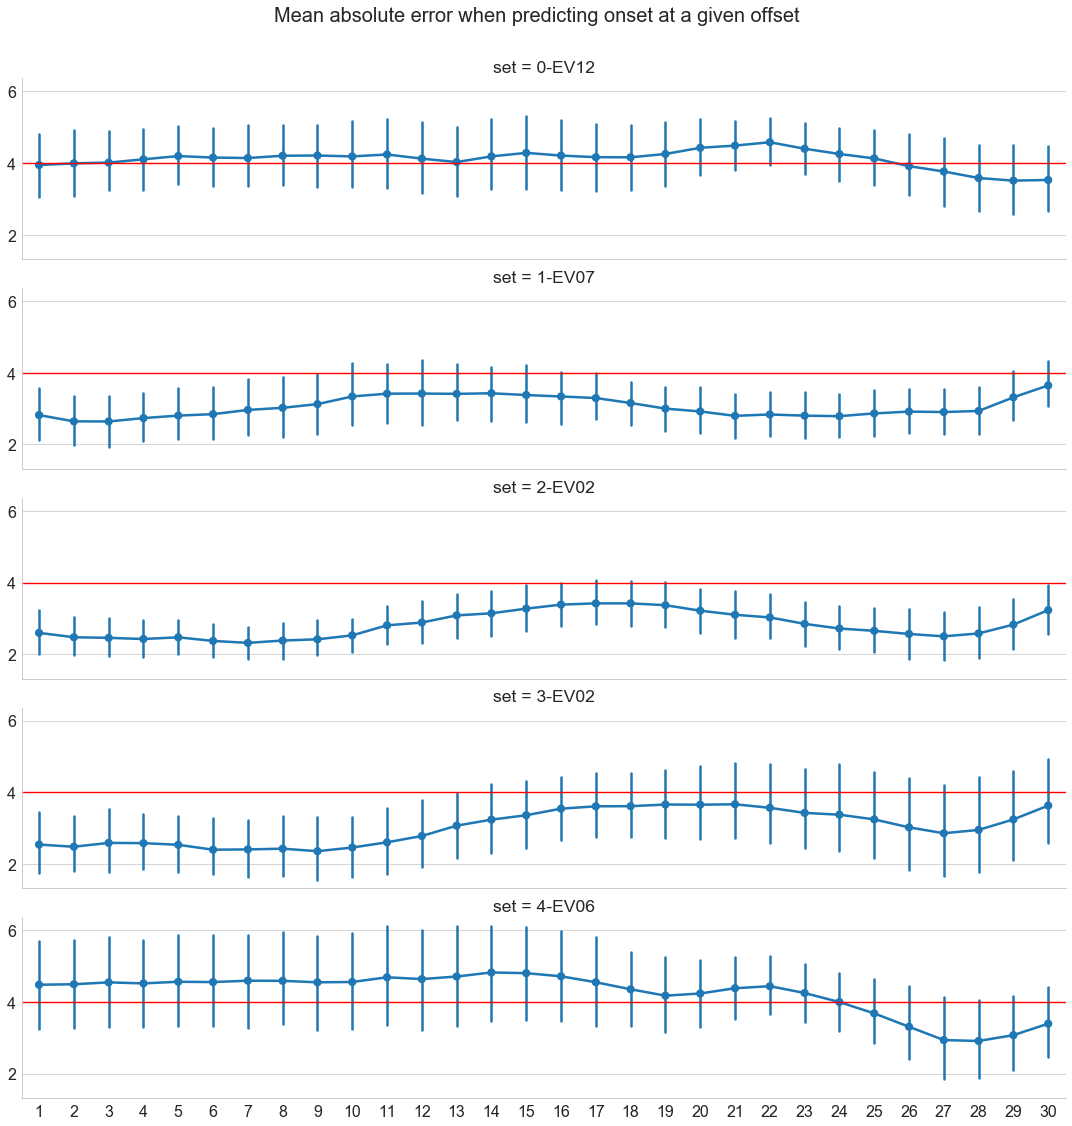
\includegraphics[width=\linewidth]{./99_appendix/img/prediction_accuracy_offset_split.png}
  \caption{Mean-absolute error (with 0.95 CI) of each offset from MoK, averaged over the predictions of the final experiments on the test set (1985, 1995, 2003, 2004, 2005, 2014, 2015, 2017).}
  \label{apx:prediction_accuracy_offset_ci}
\end{figure}

\begin{figure}[h]
  \centering
  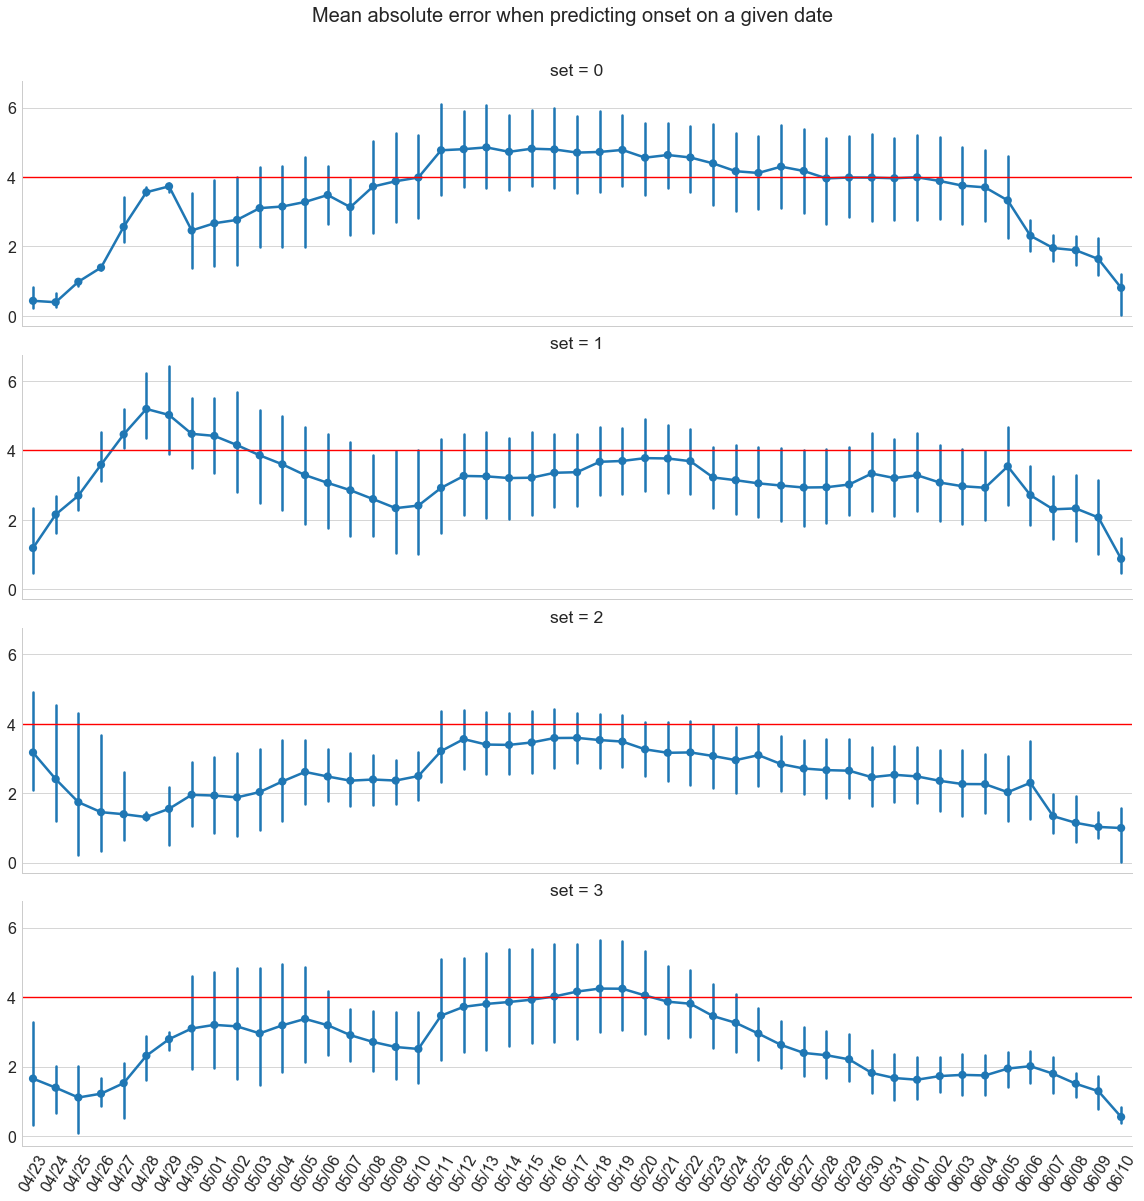
\includegraphics[width=\linewidth]{./99_appendix/img/prediction_accuracy_dates_split.png}
  \caption{Mean-absolute error (with 0.95 CI) of each prediction date previous to MoK, averaged over the predictions of the final experiments on the test set (1985, 1995, 2003, 2004, 2005, 2014, 2015, 2017).}
  \label{apx:prediction_accuracy_dates_ci}
\end{figure}
